\documentclass[]{article}
\usepackage{lmodern}

\usepackage{etoolbox}
\usepackage{graphicx}
\usepackage{marginnote}
%\usepackage[usenames,dvipsnames]{color}
\usepackage[dvipsnames]{xcolor}
\usepackage{enumitem}

\usepackage{amssymb,amsmath}
\usepackage{ifxetex,ifluatex}
\usepackage{fixltx2e} % provides \textsubscript
\ifnum 0\ifxetex 1\fi\ifluatex 1\fi=0 % if pdftex
  \usepackage[T1]{fontenc}
  \usepackage[utf8]{inputenc}
\else % if luatex or xelatex
  \ifxetex
    \usepackage{mathspec}
    \usepackage{xltxtra,xunicode}
  \else
    \usepackage{fontspec}
  \fi
  \defaultfontfeatures{Mapping=tex-text,Scale=MatchLowercase}
  \newcommand{\euro}{€}
\fi
% use upquote if available, for straight quotes in verbatim environments
\IfFileExists{upquote.sty}{\usepackage{upquote}}{}
% use microtype if available
\IfFileExists{microtype.sty}{%
\usepackage{microtype}
\UseMicrotypeSet[protrusion]{basicmath} % disable protrusion for tt fonts
}{}
\usepackage[margin=1in]{geometry}
\ifxetex
  \usepackage[setpagesize=false, % page size defined by xetex
              unicode=false, % unicode breaks when used with xetex
              xetex]{hyperref}
\else
  \usepackage[unicode=true]{hyperref}
\fi
%\usepackage[usenames,dvipsnames]{color}
\hypersetup{breaklinks=true,
            bookmarks=true,
            pdfauthor={},
            pdftitle={},
            colorlinks=true,
            citecolor=blue,
            urlcolor=blue,
            linkcolor=magenta,
            pdfborder={0 0 0}}
\urlstyle{same}  % don't use monospace font for urls
\usepackage{graphicx,grffile}
\makeatletter
\def\maxwidth{\ifdim\Gin@nat@width>\linewidth\linewidth\else\Gin@nat@width\fi}
\def\maxheight{\ifdim\Gin@nat@height>\textheight\textheight\else\Gin@nat@height\fi}
\makeatother
% Scale images if necessary, so that they will not overflow the page
% margins by default, and it is still possible to overwrite the defaults
% using explicit options in \includegraphics[width, height, ...]{}
\setkeys{Gin}{width=\maxwidth,height=\maxheight,keepaspectratio}
\setlength{\parindent}{0pt}
\setlength{\parskip}{6pt plus 2pt minus 1pt}
\setlength{\emergencystretch}{3em}  % prevent overfull lines
\providecommand{\tightlist}{%
  \setlength{\itemsep}{0pt}\setlength{\parskip}{0pt}}
\setcounter{secnumdepth}{0}

\author{}
\date{\vspace{-2.5em}}

% Redefines (sub)paragraphs to behave more like sections
\ifx\paragraph\undefined\else
\let\oldparagraph\paragraph
\renewcommand{\paragraph}[1]{\oldparagraph{#1}\mbox{}}
\fi
\ifx\subparagraph\undefined\else
\let\oldsubparagraph\subparagraph
\renewcommand{\subparagraph}[1]{\oldsubparagraph{#1}\mbox{}}
\fi

\begin{document}

\hypertarget{paleo-example}{%
\section{Meta-analysis arbitrary example: the `Paleo
diet'}\label{paleo-example}}

Introduction and discussion

\begin{quote}
Summarize the evidence base for the effectiveness of the Paleo diet in
reducing obesity (as measured by waist circumference). Please cover: a)
the basics of the intervention being studied; b) the research
methodology; c) the results.
\end{quote}

\begin{quote}
What is your conclusion on how effective the Paleo diet is at reducing
waist circumference? What do you regard as the key strengths and
limitations of the evidence and why?
\end{quote}

\begin{quote}
Briefly, what are the major uncertainties in your analysis? How could
your conclusion be wrong? This will likely involve saying what you
explicitly chose not to do and what you do not know.
\end{quote}

There is some evidence supporting the claim that the `Paleo diet'
reduces obesity as measured by waist circumference, at least for certain
targeted groups relative to certain 'standard recommended diets. At
least a small set of randomized trials have concluded that participants
in the ``Paleo diet treatment'' groups reduced their waist circumference
more than those in control groups.

This evidence is summarized in the meta-analysis of
@manheimerPaleolithicNutritionMetabolic2015a who report:

\begin{quote}
The Paleolithic diet resulted in greater short-term improvements in
metabolic syndrome components than did guideline-based control diets.
The available data warrant additional evaluations of the health benefits
of Paleolithic nutrition.
\end{quote}

More recent meta-analyses in reputable journals have also found
favorable results (@ghaediEffectsPaleolithicDiet2019,
@demenezesInfluencePaleolithicDiet2019a).

According to
\href{www.scimagojr.com}{https://www.scimagojr.com/journalrank.php?category=2916},
American Journal of Clinical Nutrition
(@manheimerPaleolithicNutritionMetabolic2015a) ranked second among
Nutrition and Dietetics journals, Advances in Nutrition
(@ghaediEffectsPaleolithicDiet2019) is ranked fourth, and Nutrition
Journal (@demenezesInfluencePaleolithicDiet2019a) is ranked 35th.

However, the Paleo diet remains controversial; it is still referred to
as a `fad diet' on
\href{https://en.wikipedia.org/wiki/Paleolithic_diet}{Wikipedia}
(accessed 20 Dec 2020), which claims `there is no good evidence that
following a paleolithic diet lessens the risk of cardiovascular disease
or metabolic syndrome'.*

* However, this Wikipedia article references
{[}@ghaediEffectsPaleolithicDiet2019;
@manheimerPaleolithicNutritionMetabolic2015{]}; both of these
meta-analysis would more accurately be characterized as stating that
there is some evidence but the results are not yet definitive.

{[}@fentonPaleoDietStill2016{]} criticized the
@manheimerPaleolithicNutritionMetabolic2015a meta-analysis, arguing it
overstated the findings and citing limitations of the included original
studies. ***

*** While I agree with some of the conceptual issues
{[}@fentonPaleoDietStill2016{]} raise, I find their criticism of the
statistics a bit imprecise as well as arbitrary in citing statistical
norms without justification. I return to these issues below.

\hfill\break

In this brief review I:

\begin{itemize}
\item
  \protect\hyperlink{conceptual}{Consider conceptual issues in defining
  and measuring the `impact of a diet' through standard study
  methodologies}
\item
  {[}Focus (as suggested) on the meta-analysis of
  @manheimerPaleolithicNutritionMetabolic2015a considering its methods,
  findings, and limitations{]}(\#limitations-p),

  \begin{itemize}
  \tightlist
  \item
    considering key conceptual and statistical issues,
  \item
    considering the {[}critiques of @fentonPaleoDietStill2016 and
    Manheimer's responses{]}(\#critiques), as well as other evaluations
    of this meta-analysis,
  \item
    weighing this evidence in light of a (shallow survey of) the
    consensus and other meta-analyses.
  \end{itemize}
\item
  \protect\hyperlink{boers}{Assess a particularly promising study}
  {[}@boersFavourableEffectsConsuming2014{]} (incorporated into
  @manheimerPaleolithicNutritionMetabolic2015a)
\end{itemize}

\emph{Disclaimers:} (See \protect\hyperlink{limitations}{`limitations'}
below).

\hypertarget{conceptual}{%
\subsection{Conceptual: Thoughts on nutritional studies and
meta-analysis issues}\label{conceptual}}

\hypertarget{compliance}{%
\subsubsection{Limited compliance; `what are we aiming to measure and
why?'}\label{compliance}}

Randomized controlled trials on nutrition and diet have important
limitations not faced by many other medical RCTs, such as drug trials.

Another important limitation: ``RCTs of dietary interventions cannot be
controlled with true placebos, but rather with certain constraints on
nutrient compositions, food groups, or dietary patterns''
@schwingshacklPerspectiveNutriGradeScoring2016. They also cite ``lack of
double blinding\ldots{} crossover bias, and high dropout rates'';
although dropout (attrition) is not an exclusive problem for dietary
studies.

\emph{Limited compliance} is a particularly important issue: not all
participants who are assigned to a particular diet will carefully follow
this diet. There are ways of \emph{tracking} compliance
(e.g.~``Diet-associated biomarkers'' such as 24-hour urine checks, which
are highly-rated by @schwingshacklPerspectiveNutriGradeScoring2016's
Nutrigrade). There are also ways of encouraging and incentivizing
compliance, such as providing free food (as in
@boersFavourableEffectsConsuming2014).

However, our consideration of this issue depends on what exactly itis we
want to measure, and for what purpose. For example may want to consider
either, what I will call\ldots{} *

* Note that my terminology below comes from the ``treatment effect''
literature in statistics and econometrics, with some slight abuses of
terminology. See, e.g., @angristIdentificationEstimationLocal1995.

\begin{enumerate}
\def\labelenumi{\arabic{enumi}.}
\tightlist
\item
  ``Average Treatment Effect (ATE)'': The difference in some medical
  outcome, averaged over the population of interest\ldots{} for the
  `Treatment diet' if consumed exactly as proposed relative to a
  `Control diet.'**
\end{enumerate}

** Even here, there may be some ambiguities that need to be clarified.
Should these diets specify exact amounts/calories consumed
(`isocaloric'), or only the types of foods, allowingconsumption as
desired? Do we need to ensure that other patterns, such as exercise, are
held constant across diets? (One might imagine that with random
treatment exercise patterns will be identical on average, however, some
diet may give people more energy to do exercise. We need to decide
whether this is part of the effect we wish to consider.)

\emph{or the}

\begin{enumerate}
\def\labelenumi{\arabic{enumi}.}
\setcounter{enumi}{1}
\tightlist
\item
  ``Intention to Treat (ITT)'' effect: The difference in some medical
  outcome, averaged over the population of interest\ldots{} for those
  \emph{assigned} to the treatment diet relative to the control diet.
\end{enumerate}

The ATE measure would seem to be more relevant:

\begin{itemize}
\tightlist
\item
  if we want to get at basic biological mechanisms or
\item
  if we believe we should recommed a `best diet' without adjusting for
  compliance. *
\end{itemize}

E.g., perhaps we are making recommendations for a context where
compliance is not particularly difficult (e.g.~perhaps school or
military meals). It may also be reasonable to assume that people reading
our analysis (e.g., dieters), will already make these self-control
considerations themselves, and simply wish to know which diet would ve
best, if they could live up to it.

On the other hand the ITT measure might be more relevant if we want to
consider which diet to propose ``for real people to achieve their best
outcomes.'' However:

\begin{itemize}
\item
  while the impact of the diet itself (the ATE) might be expected to be
  fairly uniform, as the basic biological mechanisms will be similar for
  similar groups of people,
\item
  I would expect that the ITT measure to have more heterogeneity and
  variation, as compliance with a particular diet might be expected to
  vary greatly for a variety of psychological and cultural/lifestyle
  reasons.
\end{itemize}

Thus the ITT may be more sensitive to the representativeness of our
sample of dieters. Given self selection and other issues, it may be
extremely difficult to recruit a ``nationally representative'' sample of
the targeted group.

In the discussion of @manheimerPaleolithicNutritionMetabolic2015, it is
not clear to me which measure of the studies are targeting. The
discussion (``whether Paleolithic \emph{nutrition} has any effect in
improving metabolic risk factors'', emphasis added) seems to suggest
that they are considering the ATE. However most of the designs seem to
involve simply different \emph{recommendations} for treatment and
control groups; these would seem much more likely to pick up the ITT for
their study sample.

\hypertarget{control-group-what-is-being-measured}{%
\subsubsection{Control group: what is being
measured?}\label{control-group-what-is-being-measured}}

(Time-permitting, I would more carefully consider which `control group'
diets are being administered or recommended.)

\hfill\break

\hypertarget{what-is-being-tested-and-how-broadly-should-we-interpret-the-results}{%
\subsubsection{What is being tested and how broadly should we interpret
the
results?}\label{what-is-being-tested-and-how-broadly-should-we-interpret-the-results}}

Broadly, the Paleo diet involves:

\begin{enumerate}
\def\labelenumi{\arabic{enumi}.}
\item
  Multiple differences relative to more traditional diets
\item
  A series of connected claims about the \emph{mechanism} by which it
  achieves benefits, and about nutrition and health in general
\end{enumerate}

\hfill\break

It is important to note that even if there is clear evidence that
(recommending or implementing) the `Paleo diet' causes positive health
benefits relative to an older diet:

\begin{enumerate}
\def\labelenumi{\arabic{enumi}.}
\item
  There is some inconsistency and much heterogeneity in the definition
  of the Paleo diet, as noted by @zazpeScopingReviewPaleolithic2020, who
  propose a particular `PaleoDiet' score
\item
  We don't know \emph{which} of the components of the Paleo diet were
  beneficial (some may even have been harmful, but outweighed by others
  which were even more strongly beneficial.
\item
  We don't have evidence that narrowly supports the claims made by Paleo
  advocates. Even if elements of the Paleo diet are beneficial, it may
  be through other mechanisms and channels than those proposed.
\end{enumerate}

\hypertarget{manheimer}{%
\subsection{Manheimer et al}\label{manheimer}}

\hypertarget{strengths-and-limitations}{%
\subsubsection{Strengths and
limitations}\label{strengths-and-limitations}}

The authors follow standard protocols and recommendations. However,
these systems themselves may merit some further examination.*

* E.g., I would like to better understand how the GRADE system used to
asses the quality of evidence has \emph{determined} the weights for
different categories of `quality' chosen. @Quintana2015 note ``there are
more than 80 tools available to assess the quality and risk of bias in
observational studies''\ldots{} Perhaps there are a similar number of
tools for RCT studies.

They have:

\begin{enumerate}
\def\labelenumi{\arabic{enumi}.}
\tightlist
\item
  Prospectively (in advance) {[}registered their protocol with
  PROSPERO{]}(\url{http://www.crd.york.ac.uk/PROSPERO/*/}*

  ** This reduces the risk of ``hypothesizing after the results are
  known'' \ldots{} `HARKing' @kerrHARKingHypothesizingResults1998", as
  noted by @Quintana2015. However it is difficult to verify when a
  meta-analysis was actually started, even privately. Here
  pre-registration partially depends on an honor and trust system.
\item
  Searched a broad collection of appropriate databases:
\end{enumerate}

\begin{itemize}
\tightlist
\item
  both literature databases such as PubMed
\item
  and databases of clinical trials
\end{itemize}

They also claim to have contacted ``experts in the field'' (these should
have been named) to consider whether any trials had been overlooked.
This seems to have been a well-planned and adequate search, not
neglecting the ``gray literature'' (@paezGrayLiteratureImportant2017)
and limiting ``file drawer'' bias (@kennedyOldFiledrawerProblem2004).
They carefully explained their selection method, and illustrated it in a
flow diagram.

\begin{enumerate}
\def\labelenumi{\arabic{enumi}.}
\setcounter{enumi}{2}
\item
  Broadly assessed the quality of the evidence following the GRADE
  protocol, finding the overall evidence to be of `moderate' quality
  (for waist circumference).
\item
  Analyzed the overall evidence using a frequentist Random-Effects
  model, estimating both a mean effect and a heterogeneity term. I find
  this approach to be reasonably appropriate, but I would prefer a
  \emph{Bayesian} meta-analysis.
\item
  Plotting the evidence for each outcome with the standard recommended
  tree plots, clearly depicting the (frequentist) confidence intervals
  for each study and overall.
\end{enumerate}

\textbf{Presentation, transparency and characterization}: My general
impression is that they have clearly and cleanly stated their approach
and methods, and reasonably characterized their findings, without
overstatement.* E.g., they write:

\begin{quote}
Although there is moderate quality evidence from randomized controlled
intervention studies to suggest that the Paleolithic diet can improve
metabolic syndrome components, we believe that more studies are required
before Paleolithic nutrition can be recommended in future guidelines.
(p.~928).
\end{quote}

* However, I would have liked to see their code and data made available,
or at least more prominently noted (I may have overlooked it).

\hypertarget{limitations}{%
\paragraph{Limitations}\label{limitations}}

\begin{enumerate}
\def\labelenumi{\arabic{enumi}.}
\tightlist
\item
  Small number of studies, small sample, wide confidence intervals
\end{enumerate}

\begin{quote}
Four RCTs that involved 159 participants were included. The 4 control
diets were based on distinct national nutrition guidelines but were
broadly similar.
\end{quote}

As the authors acknowledge, this is a small number of studies and the
sample as a whole is rather small. This leads to fairly wide confidence
intervals by most measures.

As noted below, the evidence does not allow us to rule out heterogeneity
across studies. With only a few studies presented, we do not have good
sense of how robust these results would be to considering other
populations, control diet comparisons, etc.

\begin{center}\rule{0.5\linewidth}{0.5pt}\end{center}

This suggests the limitations of the evidence, not a weakness of the
authors' analysis. To me their inclusion criteria seem reasonable. I
agree, e.g., with their decision that:

\begin{quote}
Crossover RCTs were eligible for inclusion, but we used data from only
the first phase before the crossover occurred because we considered the
risk of carryover effects to be high
\end{quote}

However, particularly in line with the points made in
@schwingshacklPerspectiveNutriGradeScoring2016, I would like to see a
meta-analysis considering not only RCTs but also other reasonable
approaches, such as cohort studies.

\begin{center}\rule{0.5\linewidth}{0.5pt}\end{center}

\begin{enumerate}
\def\labelenumi{\arabic{enumi}.}
\setcounter{enumi}{1}
\tightlist
\item
  Possible signs of authors' pre-judgement and funding pressure
\end{enumerate}

\begin{itemize}
\tightlist
\item
  The study was `Supported in part by the National Center for
  Complementary and Alternative Medicine of the US NIH (grant R24
  AT001293; EWM)', a group that I might suspect to be somewhat
  sympathetic to the anti-establishment linked `back to nature'
  philosophy of the Paleo diet.
\end{itemize}

\hypertarget{overall-results-interpretation-consideration-of-evidence-presented-in-manheimerpaleolithicnutritionmetabolic2015}{%
\subsubsection{Overall results, interpretation, consideration of
evidence presented in
@manheimerPaleolithicNutritionMetabolic2015}\label{overall-results-interpretation-consideration-of-evidence-presented-in-manheimerpaleolithicnutritionmetabolic2015}}

I reproduce the most relevant part of
@manheimerPaleolithicNutritionMetabolic2015's results below:

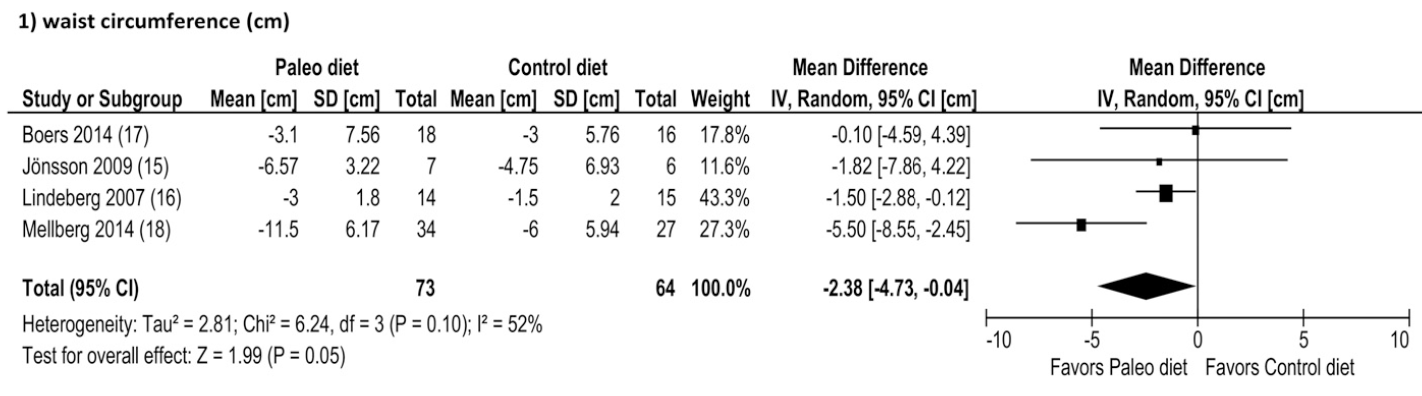
\includegraphics{waist_manheim.png}

In the individual studies, the Paleo diet participants reduced their
waist circumference (`WC') by an average of 3-11cm, with some
differences across studies. For control diet participants the reduction
was between 3 and 6 cm on average. The `difference in loss' ranged from

\begin{itemize}
\tightlist
\item
  a virtual zero with a 95\% confidence interval of {[}-4cm, +4cm{]} in
  Boers et al (the study where food was provided)
\item
  to a 5.5 cm greater loss for Paleo diets (in Mellberg et al).
\end{itemize}

The reported meta-analytic estimate is an average of 2.38 cm greater
loss in Paleo relative to the control diet, with a 95\% confidence
interval {[}-4.73, -0.04{]}, thus a `just significant' difference at the
standard NHST threshold of \(p<0.05\).

\hfill\break

\emph{Does this imply a large relative effect of Paleo?} \emph{Does it
bound the effect as `small at best'}?

To consider the magnitude of an effect such as this, it is helpful to
consider overall averages and spreads. The average US male WC is roughly
102 cm (@fryarMeanBodyWeight2018) and 98 cm for women\ldots*

I could not quickly find a reputable source for averages in Sweden and
Netherlands, where most of the studies were conducted, but
\href{https://www.dailymail.co.uk/health/article-2441250/Average-BMI-Artist-compares-sizes-men-various-countries.html}{secondhand
reports} suggest it is somewhat smaller, perhaps 90 cm.

\ldots{} which (for men) is also approximately the
\href{https://www.heart.org/en/health-topics/metabolic-syndrome/about-metabolic-syndrome}{threshold
circumference considered a risk factor for metabolic syndrome} (accessed
29 Dec 2020). I quickly, (and perhaps incorrectly) imputed a
standard-deviation of roughly 52 cm.**

** Drawing from @fryarMeanBodyWeight2018 statistics, I multiplied the
square root of the reported sample size (\(\sqrt(43169 )\)) by the
reported standard error of 0.1 (for the table in inches, the figure in
the centimeter table didn't make sense), and converted back to cm. This
calculation may be incorrect; I would like to check it, or better still,
find some scientific estimates of dispersion measures for this (SD,
quantile, IQR, etc.) I would also like to read more about what WC losses
are considered normal, reasonable, and substantial in this context.

\hfill\break

\textbf{Heterogeneity}

The evidence also suggest between-study heterogeneity; at least we do
not have strong evidence that would allow us to rule this out. Prima
facie, we see strong differences between the studies. In particular, the
one study with a strongly different methodology (Boers et al), finds a
much smaller (near-zero effect). In their formal measures, we see an
\(I^2\) of 52\%, conventionally classified as ``moderate
heterogeneity''. I believe \(\tau^2 of 2.81\) can be interpreted as a
`standard deviation in true effect size between studies' of \(\tau =\)
1.6763055, which seems, again, `moderate'.***

*** I suspect that if we allowed a variety of other methods of
estimating and reporting this (including Bayesian) and we reported the
confidence/credible intervals on this between-study variance, the
results might suggest the possibility of more substantial heterogeneity.

Although the NHST for heterogeneity is not significant by standard
measures (\(P=0.10\)), a simple `failure to reject in a diagnostic test'
does not constitute substantial reason to ignore a potentially-important
concern.*

A `failure to reject the null' is not in itself, strong evidence for the
null hypothesis. Among other things, I suspect a lack of power to detect
heterogeneity with only four studies.

\hypertarget{my-rough-conclusions-from-manheimer-et-al}{%
\subsubsection{My rough conclusions from Manheimer et
al}\label{my-rough-conclusions-from-manheimer-et-al}}

\begin{enumerate}
\def\labelenumi{\arabic{enumi}.}
\item
  The above evidence suggests some relative benefit of the Paleo diet,
  but not an extremely large benefit. To the extent
\item
  These (3) studies that find greater benefits are ones where compliance
  is particularly important, while the one study where food is provided
  (isocaloric for both diets) Does not seem to find a benefit. This
  casually suggests that `easier compliane' may be one of the major
  benefits of the Paleo diet relative to a traditional diet, but
  obviously, more evidence would be needed to support this conclusion.
\end{enumerate}

\hypertarget{critiques}{%
\subsubsection{External critiques and evaluations of Manheimer et al,
(esp Fenton) authors' response}\label{critiques}}

{[}@fentonPaleoDietStill2016{]}'s critique of
@manheimerPaleolithicNutritionMetabolic2015's focal statistical
comparisons appears to result from a mis-reading.*

``We did not report separate tests against baseline within groups as
Fenton and Fenton suggest but rather a comparison of the differences in
change from baseline between groups.'' {[}@manheimerReplyTRFenton2016{]}

@schwingshacklPerspectiveNutriGradeScoring2016 develops the `Nutrigrade'
scoring system for the strength of the evidence presented in a
meta-analysis, specifically for nutrition research.*

* Note that these scores are not a verdict on the quality of the
meta-analysis itself but of the evidence strength presnted within.

Their system and relative points system was independently developed; a
major point of contrast with GRADE (@guyattGRADEEmergingConsensus2008)
seems to be Nutrigrade's greater valuation of cohort studies relative to
RCTs, reflecting some of the rationales mentioned above, such as
\protect\hyperlink{compliance}{limited compliance}. They `Nutrigrade'
the evidence in @manheimerPaleolithicNutritionMetabolic2015 as 5.75, or
`Low', explained as ``there is low confidence in the effect estimate;
further research will provide important evidence on the confidence and
likely change the effect estimate.'' Of 10 randomly meta-analysis
studies they rated, this was the fifth-highest `Nutrigrade'.

Overall, the `reviews' of the strength of evidence meta-analysis are
fair to middling. All, including the original authors, seem to agree
that the ``the current evidence on the paleo diet might be considered
early or preliminary and that further research is critically needed''
(@manheimerReplyTRFenton2016), although there seems to be some
disagreement about how promising an avenue this is for further inquiry.

\hypertarget{other-meta-analyses-and-consideration-of-the-paleo-diet}{%
\subsection{Other meta-analyses and consideration of the Paleo
diet}\label{other-meta-analyses-and-consideration-of-the-paleo-diet}}

As noted, the Paleo diet is controversial and not widely accepted in the
medical profession. As @manheimerPaleolithicNutritionMetabolic2015 note

\begin{quote}
a 2015 US News and World Report ranking of 35 diets with input from a
panel of health experts placed the Paleolithic diet dead last, citing a
lack of research evidence that showed clinical benefits.
\end{quote}

However, more work also seems to support a claim such as `recommending
the Paleo diet is succesful in reducing waist circumference in the
short-term, relative to recommending more traditional diets.'

In particular, @ghaediEffectsPaleolithicDiet2019 perform a meta-analysis
of eight RCT studies (the four considered by Mannheimier et al, plus
four more that were conducted since 2015) and find ``a {[}Paleo diet{]}
significantly reduced \ldots{} waist circumference (WMD = −2.90 cm; 95\%
CI: −4.51, −1.28 cm)''. These results are rather similar to those of
@manheimerPaleolithicNutritionMetabolic2015. Time-permitting, I would
like to examine this meta-analyis in more detail.

\hypertarget{process-of-finding-relevant-work-informal}{%
\subsubsection{Process of finding relevant work
(informal)}\label{process-of-finding-relevant-work-informal}}

\emph{Notes}: In the limited time I had available, I did some keyword
searches on Google scholar, such as
\texttt{\textquotesingle{}paleo\ diet\textquotesingle{}\ AND\ \textquotesingle{}meta-analysis}`\texttt{and}paleo
diet\texttt{AND}randomized controlled trial` I also followed a
'snowball' approach to consider which studies were cited, and which
studies cited @manheimerPaleolithicNutritionMetabolic2015, and the
papers most prominently cited within. I did not do the systematically
nor did I keep track of my process (as I would do if I were doing this
more seriously, e.g., for my own meta-analysis).

\hypertarget{boers}{%
\subsection{Focus: Boers et al}\label{boers}}

Unlike the other trials considered in
@manheimerPaleolithicNutritionMetabolic2015,
@boersFavourableEffectsConsuming2014 ``provided home-delivered
Paleolithic and control diet meals to participants''. This permits a
more direct examination of what I called the
\protect\hyperlink{compliance}{ATE}. I expect this effect to be less
variable and more generalizable across populations, because issues of
differential compliance will be reduced.

This study is also particular strong because it has (apparently) a zero
attrition rate (`34/34 analyzed'), while attrition in the other cited
studies is substantial. Particular forms of non-random attrition can
strongly bias estimated treatment effects, biasing both the ATE and ITT
mentioned above.*

* See @leeTrainingWagesSample2009 for a clear discussion of this, as
well as an approach to `bounding this bias' under a particular
monotonicity assumption.

\hypertarget{overall-analysis}{%
\subsection{Overall analysis}\label{overall-analysis}}

My overall impression from the above is that the meta-analytic results
do suggest some benefit of the Paleo diet in reducing waist
circumference for groups that are vulnerable to the metabolic syndrome.

However:

\begin{itemize}
\item
  The evidence plausibly suggests that the benefit of this diet comes
  largely through greater adherence, rather than through a direct
  nutritional advantage. Perhaps, as is popular conventional wisdom
  ``eating more proteinssimply makes it easier to feel full and thus not
  overeat''.
\item
  The studies I have seen compare the diet only to a traditional diet,
  rather than to another low carbohydrate diet. Thus, I do not see any
  strong evidence that the Paleo diet offers advantages (or
  disadvantages) over, e.g., the `South Beach' or `Keto' diets. Thus the
  evidence does not support (nor refute) \emph{mechanism and diet
  philopsophy} behind Paleo.\\
\end{itemize}

Furthermore, there also appears to be \textbf{limited evidence}; I am
not highly confident in even the above claim. I did not see aa wide
array of high-quality studies evaluating the Paleo diet for the relevant
large and diverse populations in natural settings.

\hypertarget{limitations-p}{%
\subsubsection{Limitations and uncertainties to my own analysis;
proposed future steps}\label{limitations-p}}

\begin{quote}
Briefly, what are the major uncertainties in your analysis? How could
your conclusion be wrong? This will likely involve saying what you
explicitly chose not to do and what you do not know.
\end{quote}

\textbf{Caveats:} I am an economist, not a nutritionist or a life
scientist. While I am working to build up my expertise in this area I
have only limited experience conducting and for evaluating
meta-analyses. The evaluation here was only a limited and shallow
exercise done in a 10 hour window for a specific purpose. I did not do a
broad and systematic review of the literature.

I was only able to take a narrow focus for this exercise, mainly
considering
\href{mailto:only@manheimerPaleolithicNutritionMetabolic2015}{\nolinkurl{only@manheimerPaleolithicNutritionMetabolic2015}}
review, as well as some connected work. To gain a more reliable answer
to this question, there are a number of further , involving gaining
better understanding, digging deeper into the data and analysis, and
consulting a range of experts.

\hfill\break

\textbf{Some steps I would take}

\begin{enumerate}
\def\labelenumi{\arabic{enumi}.}
\tightlist
\item
  Better understand: \emph{What is the relevant question?}
\end{enumerate}

As I suggested above, the nature of evidence that is appropriate will
depend on what question is being asked, and what purpose this is being
put to. Why do we care about the answer to this? Are we considering
recommending this diet to a particular population? How strong
incentive/food provision will we be able to provide? Are we deeply
interested in the biological mechanisms or the behavioral ones? What do
we intend to do with the results of this analysis, i.e., what policy
choices will it inform?

If I had better answers to question like these, I would know which types
of studies to focus on, and how to better consider their results.

\begin{enumerate}
\def\labelenumi{\arabic{enumi}.}
\setcounter{enumi}{1}
\tightlist
\item
  Pursue a more systematic consideration of the literature and evidence
\end{enumerate}

\begin{itemize}
\tightlist
\item
  documenting my protocol
\item
  carefully considering which fields and subfields to focus on
\item
  discussing my approaches with experts in these fields, seeking their
  consideration of the points I have made in this essay
\end{itemize}

\begin{enumerate}
\def\labelenumi{\arabic{enumi}.}
\setcounter{enumi}{2}
\tightlist
\item
  Pursue a better understanding of
\end{enumerate}

\begin{itemize}
\item
  the reasoning behind standardized protocols for meta-analysis and
  `bias-assessment', consulting, e.g., the
  \href{https://training.cochrane.org/handbook/current}{`Cochrane
  Handbook for Systematic Reviews of Interventions'}
\item
  How nutritionists and dieticians differentiate (what I call above) the
  ITT and ATE
\item
  The argument for particular meta-analytic approaches in nutrition and
  health studies (in comparison to my area of greater expertise,
  economics and social science)
\end{itemize}

\hfill\break

\begin{enumerate}
\def\labelenumi{\arabic{enumi}.}
\setcounter{enumi}{3}
\tightlist
\item
  More closely inspect and evaluate
\end{enumerate}

\begin{itemize}
\tightlist
\item
  @manheimerPaleolithicNutritionMetabolic2015's code used for doing the
  (frequentist) Random-effects meta-analysis, to understand the specific
  inclusion, variable-coding, and estimator choices, and the sensitivity
  of the results to this.*
\end{itemize}

* For example, as explained in the excellent tutorial
@harrerDoingMetaanalysisHandson2019Mathias,
\href{https://bookdown.org/MathiasHarrer/Doing_Meta_Analysis_in_R/random.html\#tau2}{there
are a range of popular estimators for \(\tau^2\)}, the variance of the
distribution of true effect sizes. There is also some debate over
whether random effects is appropriate, particularly because of its
sensitivity to small studies.

\begin{itemize}
\item
  The particularly promising @boersFavourableEffectsConsuming2014 study
  as \protect\hyperlink{boers}{noted above}
\item
  @ghaediEffectsPaleolithicDiet2019, and
  @demenezesInfluencePaleolithicDiet2019a, and any other promising
  analyses that come from the aforementioned systematic literature
  survey
\end{itemize}

\end{document}
